\chapter{Die Basics}
\pagestyle{empty}

Im Ersten Kapitel werden wir die Grundlagen der Programmierung lernen.

Wir werden rausfinden, was ein Compiler ist, wie ein Programm abläuft und wie man es startet. Wir werden Benutzereingaben verarbeiten und Ausgaben an den Benutzer geben. Wir lassen den Computer Rechnungen für uns anstellen und lernen, was der Kontrollfluß ist - und wie man ihn beeinflusst. Zuletzt werden wir Arrays kennenlernen und unser erstes nützliches Progamm schreiben.

\lesson{Hello world}

Die erste Lektion beschäftigt sich alleine mit der Frage, was eigentlich eine
Programmiersprache überhaupt ist und wie wir den Computer dazu bringen können,
daraus etwas zu machen, was er ausführen kann.  In guter alter
Programmiertradition tun wir das an dem simpelsten aller Programme: Einem, was
einfach nur ein „Hallo Welt!“ ausgibt.

Wie bringen wir also den Computer dazu, diese Ausgabe zu generieren? Dass er
keine natürliche Sprache versteht, sollte klar sein - intern besteht er aus
lauter Transistoren (wenn ihr nicht wisst, was das ist, denkt an winzige
Schalter), die nur die Zustände „an“ und „aus“ kennen, wir müssen also die
Anweisung „gebe Hallo Welt aus“ in ein Format übersetzen, was nur „an“ und
„aus“ benutzt.

Früher wurde genau dies benutzt - meistens über Lochkarten, die vom Computer
gelesen wurden, „ein Loch“ war dann zum Beispiel ein „an“ und „kein Loch“ war
„aus“, so wurde dann das Programm in Reihen angeordnet und jede Reihe entsprach
einem Befehl oder einem Parameter für diesen Befehl.  Dieses Format nennt sich
„Maschinensprache“ und ist immer noch das, was wir heute dem Computer
übergeben, nur, dass wir keine Lochkarten mehr benutzen, sondern Dateien, in
denen lange Ströme von codierten 0en und 1en stehen.

Nun kann man sich vorstellen, dass es ganz schön anstrengend ist, ein
umfangreiches Programm in 0en und 1en zu beschreiben. Deswegen benutzt man
heutzutage so genannte Hochsprachen, um Programme zu beschreiben. Wir
beschreiben also den Programmablauf in einer von Menschen lesbaren und
verstehbaren Sprache -- wir benutzen hier \Cpp.  Die Programmbeschreibung in
\Cpp legen wir dabei in einer Textdatei ab, meistens hat diese die Endung
\texttt{.cpp}.

Diese Beschreibung des Programms übergeben wir dann an einen \emph{Compiler},
der daraus dann Maschinencode generiert, den wir wiederum dem Computer zur
Ausführung geben können.  Der Compiler für \Cpp, den wir in diesem Kurs
benutzen wollen, heißt \texttt{g++}.

Dem Compiler übergeben wir die zu kompilierende Datei als Parameter, indem wir
sie im Terminal dahinter schreiben:
\begin{center}
\texttt{g++ zuKompilierendeDatei.cpp}
\end{center}
Wir können zusätzlich den Namen der Ausgabedatei festlegen, indem wir vor diese
ein \texttt{-o} (o für output) schreiben:
\begin{center}
\texttt{g++ -o outputDatei zuKompilierendeDatei.cpp}
\end{center}

Nachdem \texttt{g++} uns also ein Maschinencodefile \texttt{outputDatei}
erzeugt hat, können wir es zur Ausführung bringen. Wir tun das, indem wir in
einem Terminal
\begin{center}
	\texttt{./outputDatei}
\end{center}
eingeben, also einen Punkt, ein Slash und dann den Dateinamen.

Zur besseren Übersichtlichkeit hier der ganze Vorgang noch mal in einem
Diagramm:

% TODO: Buttugly, but well...
\begin{center}
    \resizebox{\textwidth}{!}{
        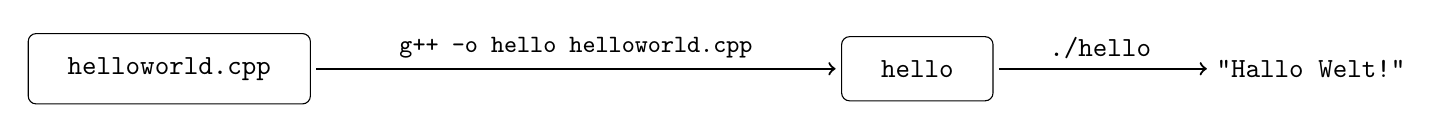
\begin{tikzpicture}
            \node (nHelloWorldCpp) [ shape=rectangle, rounded corners = 0.1cm, draw=black, inner xsep=0.5cm, inner ysep = 0.3cm ] {\texttt{helloworld.cpp}};
            \node (nHello) [ right of = nHelloWorldCpp, node distance = 9.5cm, shape=rectangle, rounded corners = 0.1cm, draw = black, inner xsep = 0.5cm, inner ysep = 0.3cm ] {\texttt{hello}};
            \draw [->, thick, shorten >= 2pt, shorten <= 2pt ] (nHelloWorldCpp) -- (nHello) node [ midway, above, font = \small ] { \texttt{g++ -o hello helloworld.cpp}} ;
            \node (nOutput) [ right of = nHello, node distance = 5cm, shape=rectangle ] {\texttt{"Hallo Welt!"}};
            \draw [->, thick, shorten <= 2pt] (nHello) -- (nOutput) node [ midway, above ] {\texttt{./hello}};
        \end{tikzpicture}
    }
\end{center}

\textbf{Praxis:}
\begin{enumerate}
	\item Öffnet ein Terminal, ihr findet dies in den Anwendungen (oben rechts)
		unter „Systemwerkzeuge“
    \item Wechselt in das Verzeichnis \texttt{vorkurs/lektion01}, indem ihr
		\texttt{cd vorkurs/lektion01}\footnote{was dieser Befehl genau tut und wie er funktioniert, erfahrt ihr in Lektion 2} eingebt und enter drückt.
    \item In diesem Verzeichnis liegt eine Datei \texttt{helloworld.cpp}.
        Benutzt \texttt{g++}, um diese zu einer Datei \texttt{hello} zu
        kompilieren. Orientiert euch dazu an den Befehlen von oben.
    \item Führt die Datei \texttt{hello} aus.
\end{enumerate}

\inputcpp{helloworld.cpp}

\textbf{Spiel:}

Ihr könnt nun versuchen, den Quellcode selbst zu verändern und damit ein wenig
herumzuspielen. Öffnet dazu einen Editor (in den Anwendungen findet ihr z.B.
unter „Zubehör“ den Editor gedit) und öffnet die Datei
\texttt{vorkurs/lektion01/helloworld.cpp}\footnote{entweder mittels
"Datei/Öffnen" in gedit oder über das Terminal mittels \texttt{gedit
helloworld.cpp}}. Denkt daran, nach jeder Änderung die Datei zu speichern und
im Terminal neu zu kompilieren und auszuführen.

Dinge, die ihr ausprobieren könntet sind zum Beispiel:
\begin{enumerate}
    \item Was passiert, wenn ihr „Hello world!“ in etwas anderes ändert?
    \item Was passiert, wenn ihr die erste Zeile löscht (der Originalquellcode
        ist in diesem pdf enthalten, ihr könnt sie also später wieder
        herstellen)?
    \item Was passiert, wenn ihr das „\verb|<< std::endl|“ löscht?
    \item Wie könnte man mehrere Sätze ausgeben? Wie könnte man mehrere Zeilen
        ausgeben?
\end{enumerate}

\lesson{Die Shell}

Wenn ihr bisher nur mit Windows oder Mac gearbeitet habt, habt ihr
wahrscheinlich in der letzten Lektion nebenbei etwas neues Kennen gelernt: Die
Shell.

Auch wenn sich unter Linux zunehmend Desktopumgebungen, wie man sie von
kommerziellen Betriebssystemen kennt verbreiten, bleibt die Shell immer noch das
Mittel der Wahl, wenn man sich mit dem System auseinander setzen, oder auch
allgemein arbeiten will. Wir erachten zumindest die Shell als wichtig genug, um
euch direkt zu beginn damit zu konfrontieren.

Wann immer ihr über das Anwendungsmenü ein Terminal startet, wird dort drin
automatisch auch eine shell gestartet. Die beiden Konzepte sind tatsächlich so
eng miteinander verknüpft, dass ihr euch um die Unterschiede erst einmal keine
Gedanken machen müsst - wann immer ihr Shell oder Terminal hört, denkt einfach
an das schwarze Fenster mit dem Text. Das ist auch das wesentliche Merkmal der
Shell, sie ist ein Textbasiertes interface zu eurem Computer. Ihr gebt Befehle
ein, sie gibt euch Text zurück und auf diese Weise könnt ihr eigentlich alles
machen, was ihr sonst gewohnterweise mit der Maus und grafischen Oberflächen
tun würdet.

Wenn die Shell auf eure Befehle wartet, zeigt sie euch den so genannten
\emph{Prompt} an. Er enthält unter anderem euren Nutzernamen und das aktuelle
Verzeichnis (\verb|~| steht dabei für euer Nutzerverzeichnis, ein spezieller
Ordner, der eurem Account zugeordnet ist und in dem ihr alle Rechte besitzt).

Wenn ihr in ein anderes Verzeichnis wechseln wollt, könnt ihr das (wie ihr
bereits in der ersten Lektion gelernt habt) mit dem Befehl \texttt{cd} tun,
gefolgt von dem Namen des Verzeichnis. Um zurück zu gehen, könnt ihr das
spezielle Verzeichnis \texttt{..} (also zwei Punkte) angeben, welches für das
nächst höher liegende Verzeichnis steht. Wenn ihr euch den Inhalt des
Verzeichnisses anschauen wollt, könnt ihr dafür den Befehl \texttt{ls}
benutzen. Um herauszufinden, in welchem Verzeichnis ihr euch befindet, könnt
ihr \texttt{pwd} nutzen, zum Kompilieren von C++-Programmen habt ihr den Befehl
\texttt{g++} kennengelernt. Solltet ihr Hilfe zu irgendeinem Befehl benötigen,
könnt ihr den Befehl \texttt{man} (für „Manual“) geben, gefolgt von dem Befehl,
zu dem ihr Hilfe braucht (über \texttt{man} werden wir später noch
ausführlicher reden).

\textbf{Praxis:}
\begin{enumerate}
    \item Öffnet ein Terminal und gebt die folgenden Befehle ein:
    \inputshell{basics.sh}
\end{enumerate}

\textbf{Spiel:}
\begin{enumerate}
    \item Versucht selbst, euer Nutzerverzeichnis (\emph{home}) zu navigieren.
        Wie viele Lektionen hat der Vorkurs?
    \item Was passiert, wenn ihr euer Homeverzeichnis verlasst (\texttt{cd ..}
        während ihr darin seid)?
    \item Versucht in der manpage von ls (\texttt{man ls}) zu stöbern und die
        verschiedenen Parameter, mit denen ihr das Verhalten steuern könnt zu
        erforschen. Findet ihr heraus, wie ihr ein longlisting anzeigen lässt,
        in dem unter anderem auch die Dateigröße zu jeder Datei steht?
\end{enumerate}

\lesson{Input und Output}

Nachdem wir ein bisschen Vertrauen in die shell entwickelt haben und zumindest
bereits unser erstes Programm kompiliert, wollen wir nun etwas spannendere
Dinge tun. Nach wie vor müsst ihr nicht jede Zeile eures Programmes verstehen.
Sollte euch bei einer bestimmten Zeile trotzdem interessieren, was genau sie
tut, versucht doch eventuell sie zu entfernen, das Programm zu kompilieren und
schaut, was sich ändert.

Wir wollen uns nun mit grundlegendem input und output vertraut machen, denn
erst wenn euer Programm mit einer Benutzerin interagiert, wird es wirklich
nützlich. Wir haben in der ersten Lektion bereits \texttt{cout} (für
\emph{console out}) kennengelernt, um Dinge auszugeben. Nun nutzen wir
\texttt{cin}, um Eingaben des Benutzers entgegen zu nehmen. Jedes Programm
unter Linux (und übrigens auch Mac OS oder Windows) kann auf diese Weise
Eingaben von der Nutzerin entgegen nehmen und Ausgaben liefern. Das ist auch
der Grund, warum die Konsole so wichtig ist und es viele Dinge gibt, die nur
mittels einer Konsole gelöst werden können: Während es viele Stunden dauert,
ein grafisches Interface zu programmieren, über die man mit dem Programm mit
der Maus kommunizieren kann, kann praktisch jeder ein textbasiertes
Konsoleninterface schreiben. Linux ist ein Ökosystem mit einer gewaltigen
Anzahl tools für jeden denkbaren Zweck und bei den meisten haben die Autorinnen
sich nicht die Mühe gemacht, extra eine grafische Oberfläche zu entwickeln.

Nun aber direkt zur Praxis:

\textbf{Praxis:}
\begin{enumerate}
    \item Öffnet die Datei \texttt{vorkurs/lektion03/helloyou.cpp} in eurem Texteditor
    \item Öffnet ein Terminal und wechselt in das Verzeichnis \texttt{vorkurs/lektion3}
    \item Kompiliert im Terminal die Datei (\texttt{g++ -o helloyou
        helloyou.cpp}) und führt sie aus (\texttt{./helloyou})
    \item Versucht verschiedene Eingaben an das Programm und beobachtet, was passiert
\end{enumerate}

\inputcpp{helloyou.cpp}

\textbf{Spiel:}

\begin{enumerate}
    \item Versucht, zu verstehen, was die einzelnen Teile des Programms tun. An
        welcher Stelle erfolgt die Eingabe? Was passiert dann damit?
    \item Erweitert das Programm um eigene Fragen und Ausgaben. Vergesst nicht,
        dass ihr das Programm nach jeder Änderung neu kompilieren und testen
        müsst.
\end{enumerate}

\lesson{Fehlermeldungen und häufige Fehler}

Wenn ihr in den vergangen Lektionen ein bisschen herumprobiert habt, wird es
euch sicher das ein oder andere mal passiert sein, dass euch der Compiler statt
eines funktionierenden Programms eine Riesenmenge Fehlermeldungen ausgespuckt
hat und ihr einen Schreck bekamt und schon dachtet, ihr hättet alles kaputt
gemacht.

\texttt{g++} ist leider bei Fehlermeldungen immer sehr ausführlich und gibt
euch lieber viel zu viel, als viel zu wenig aus. Das kann im ersten Blick ein
bisschen überwältigend wirken, aber wenn man einmal gelernt hat, wie die
Fehlermeldungen am Besten zu lesen sind, ist das alles gar nicht mehr so
schlimm.

Wir schieben deswegen eine Lektion über häufige Fehlerquellen ein und wie man
Fehlermeldungen von \texttt{g++} liest, um möglichst schnell die Ursache des
Fehlers zu finden.

Nehmen wir z.B. mal folgendes Programm:

\inputcpp{fehler1.cpp}

Wenn wir versuchen, dieses zu kompilieren, gibt uns \texttt{g++} folgendes aus:

\begin{textcode*}{label=g++ -o fehler1 fehler1.cpp}
fehler1.cpp: In function 'int main()':
fehler1.cpp:2:5: error: 'cout' is not a member of 'std'
fehler1.cpp:2:35: error: 'endl' is not a member of 'std'
\end{textcode*}

Wenn wir diese Fehlermeldung verstehen wollen, fangen wir immer ganz oben an,
egal wie viel Text uns der Compiler ausspucken mag. In diesem Fall sagt uns die
erste Zeile, in welcher Datei (\texttt{fehler1.cpp}) der Fehler aufgetreten ist
und in welcher Funktion (\texttt{int main()}). Die beiden Zeilen
danach sind sogar noch spezifischer: Sie enthalten zu Beginn den Dateinamen,
dann einen Doppelpunkt, gefolgt von einer Zeilennummer, gefolgt von einer
Spaltennummer. Das gibt euch ganz genau die Stelle an, an der der Compiler
etwas an eurem Code zu bemängeln hat. In diesen Fall ist, was der Compiler
bemängelt, dass \texttt{cout} bzw. \texttt{endl} nicht in \texttt{std} sind.
Was genau \texttt{std} bedeutet muss uns nicht interessieren, aber der Rest
sagt uns (mit ein bisschen Erfahrung) dass wir die Definition von \texttt{cout}
und \texttt{endl} nicht haben - was nicht weiter verwunderlich ist, denn diese
beiden Dinge werden in der Datei \texttt{iostream} definiert, die wir früher
immer includiert haben.

Damit wissen wir jetzt auch (endlich) was das \mint{c++}|#include <iostream>|
zu bedeuten hatte. Offenbar brauchen wir das, wenn wir Konsolen input und
output machen wollen, da es die Definitionen von \texttt{cout}, \texttt{cin},
\texttt{endl} und ähnlichem enthält.

Der nächste sehr häufig vorkommende Fehler ist subtiler:

\inputcpp{fehler2.cpp}

Wenn wir versuchen, dies zu kompilieren, bekommen wir vom Compiler
entgegengespuckt:

\begin{textcode*}{label=g++ -o fehler2 fehler2.cpp}
fehler2.cpp: In function 'int main()':
fehler2.cpp:5:1: error: expected ';' before '}' token
\end{textcode*}

Wiederum sagt uns die erste Zeile, in welcher Datei und Funktion der Fehler
aufgetreten ist. Die zweite Zeile sagt uns wo, nämlich in Zeile 5, direkt am
Anfang. Die Beschwerde des Compilers ist, dass er ein Semikolon erwartet hat,
aber eine geschlossene geschweifte Klammer gefunden hat. Der Grund dafür ist,
dass in \Cpp erwartet wird, dass jede Anweisung mit einem Semikolon abgeslossen
wird.  Wenn ihr euch die bisherigen Quellcodedateien anschaut, werdet ihr
feststellen, dass hinter den allermeisten Zeilen ein solches Semikolon steht.
Hier fehlt es allerdings nach der Ausgabe in Zeile 4. Sobald wir es hinzufügen,
beschwert sich der Compiler nicht mehr.

Hier zeigt sich eine ein bisschen verwirrende Angewohnheit von Fehlermeldungen
von \Cpp: Obwohl der Compiler behauptete, der Fehler läge in Zeile 5, lag er in
Wahrheit bereits in Zeile 4. Hier müsst ihr dem dummen Compiler ein wenig
nachsichtig sein - er kann es einfach nicht besser wissen. Wenn ihr also mal in
der richtigen Zeilennummer nachschlagt, aber nicht wisst, wo dort der Fehler
sein sollte, schaut vielleicht mal ein oder zwei Zeilen darüber, vielleicht
wusste der Compiler es einfach nicht besser.

\textbf{Praxis:}
\begin{enumerate}
    \item Versucht, folgende Dateien zu kompilieren und schaut euch die
        Fehlermeldung an. In welcher Zeile, in welcher Spalte liegt der Fehler?
        Was gibt euch der Compiler als Fehlermeldung aus?
    \item Versucht, die aufgetretenen Fehler zu korrigieren. Bekommt ihr es
        hin, dass der Compiler sich nicht mehr beschwert und das Programm
        korrekt arbeitet (schaut euch ggf. die bisher gezeigten Quellcodes an)?
\end{enumerate}

\inputcpp{fehler3.cpp}
\inputcpp{fehler4.cpp}

\textbf{Spiel:}
\begin{enumerate}
    \item Das folgende Programm enthält mehrere Fehler. Bekommt ihr trotzdem
        raus, welche das sind und könnt ihr sie beheben (Tipp: „c++ math“ zu
        \href{http://lmgtfy.com/?q=c\%2B\%2B+math}{googlen} kann euch hier vielleicht weiter bringen)?
    \item Wenn ihr in den Vergangen Lektionen ein bisschen gespielt habt und
        vereinzelnd versucht habt, Dinge zu löschen, Werden euch viele
        Fehlermeldungen begegnet sein, versucht, diese zu lesen und
        interpretieren, was euch der compiler hier sagen will.
\end{enumerate}

\inputcpp{fehler5.cpp}

\lesson{Variablen}

Das Programm \texttt{variablen.cpp} erzählt von ihrem Tag.
Compilier es und guck dir die Ausgabe an.

\inputcpp{variablen.cpp}

Da immer wieder das gleiche Wort \glqq{}wundervoll\grqq{} benutzt wird, wurde es in eine sogenannte \emph{Variable} ausgelagert.
Eine Variable ist ein Wert der mit einem Namen benannt wird.
Dabei findet die Zuweisung durch ein \cppinline{=} statt, dem Namen auf der linken Seite des Gleichheitszeichen wird der Wert auf der rechten Seite zugewiesen.
Im Programm selbst ist es dann so, als würde der Wert an der Stelle des Namens stehen.

Der Wert einer Variable kann sich im Laufe des Programmes verändern.
Durch Hinzufügen der Zeile \cppinline{beschreibung = "langweilig";} wird hinter dieser Zeile anstelle von \glqq{}wundervoll\grqq{} nun \glqq{}langweilig\grqq{} ausgegeben.
Ähnlich kann wie in \texttt{helloyou.cpp} der Wert von Variablen durch \cppinline{std::cin >> beschreibung} die Benutzerin eingeben werden.

Variablen haben immer einen bestimmten \emph{Datentypen}.
In unserem Beispiel handelt es sich um \cppinline{std::string}.
Der Datentyp wird bei dem Erstellen -- also der ersten Zuweisung -- vor dem Namen angeben.
Dieser wird benötigt, damit der Computer weiß, um was für eine Art Wert es sich handelt -- ein Text sollte anders behandelt werden als eine Zahl.
Beispielsweise kann man zwei Zahlen miteinander multiplizieren, für Texte ergibt das allerdings keinen Sinn.
In der Lektion Arithmetik lernen wir mehr über Zahlen und deren Eigenheiten.

\textbf{Praxis:}
\begin{enumerate}
    \item Was passiert, wenn ihr \cppinline{beschreibung} in Zeile 5 ein anderes Wort zuweist?
    \item Definiert eine weitere Variable und schreibt einen weiteren Satz.
\end{enumerate}

\textbf{Spiel:}
\begin{enumerate}
    \item Was passiert, wenn ihr euch im Namen einer Variable „vertippt“?
    \item Definiert euch zwei \cppinline{std::string} Variablen, weist ihnen
        irgendwelchen Text zu, versucht, sie zu addieren und das Ergebnis auszugeben.
    \item Was passiert, wenn ihr eine \cppinline{std::string} Variable definiert,
        ihr aber nichts zuweist und dann versucht, sie auszugeben?
\end{enumerate}

\include{gdb1}
\include{variables}
\include{gdb2}
\lesson{Input und Output}

Nachdem wir ein bisschen Vertrauen in die shell entwickelt haben und zumindest
bereits unser erstes Programm kompiliert, wollen wir nun etwas spannendere
Dinge tun. Nach wie vor müsst ihr nicht jede Zeile eures Programmes verstehen.
Sollte euch bei einer bestimmten Zeile trotzdem interessieren, was genau sie
tut, versucht doch eventuell sie zu entfernen, das Programm zu kompilieren und
schaut, was sich ändert.

Wir wollen uns nun mit grundlegendem input und output vertraut machen, denn
erst wenn euer Programm mit einer Benutzerin interagiert, wird es wirklich
nützlich. Wir haben in der ersten Lektion bereits \texttt{cout} (für
\emph{console out}) kennengelernt, um Dinge auszugeben. Nun nutzen wir
\texttt{cin}, um Eingaben des Benutzers entgegen zu nehmen. Jedes Programm
unter Linux (und übrigens auch Mac OS oder Windows) kann auf diese Weise
Eingaben von der Nutzerin entgegen nehmen und Ausgaben liefern. Das ist auch
der Grund, warum die Konsole so wichtig ist und es viele Dinge gibt, die nur
mittels einer Konsole gelöst werden können: Während es viele Stunden dauert,
ein grafisches Interface zu programmieren, über die man mit dem Programm mit
der Maus kommunizieren kann, kann praktisch jeder ein textbasiertes
Konsoleninterface schreiben. Linux ist ein Ökosystem mit einer gewaltigen
Anzahl tools für jeden denkbaren Zweck und bei den meisten haben die Autorinnen
sich nicht die Mühe gemacht, extra eine grafische Oberfläche zu entwickeln.

Nun aber direkt zur Praxis:

\textbf{Praxis:}
\begin{enumerate}
    \item Öffnet die Datei \texttt{vorkurs/lektion03/helloyou.cpp} in eurem Texteditor
    \item Öffnet ein Terminal und wechselt in das Verzeichnis \texttt{vorkurs/lektion3}
    \item Kompiliert im Terminal die Datei (\texttt{g++ -o helloyou
        helloyou.cpp}) und führt sie aus (\texttt{./helloyou})
    \item Versucht verschiedene Eingaben an das Programm und beobachtet, was passiert
\end{enumerate}

\inputcpp{helloyou.cpp}

\textbf{Spiel:}

\begin{enumerate}
    \item Versucht, zu verstehen, was die einzelnen Teile des Programms tun. An
        welcher Stelle erfolgt die Eingabe? Was passiert dann damit?
    \item Erweitert das Programm um eigene Fragen und Ausgaben. Vergesst nicht,
        dass ihr das Programm nach jeder Änderung neu kompilieren und testen
        müsst.
\end{enumerate}

\include{arithmetic}
\include{conditionals}
\include{switch}
\include{while}
\include{for}
\lesson{Arrays}

Als nächstes wichtiges Konzept in \Cpp werden wir uns \emph{Arrays} anschauen.
Arrays sind eine Möglichkeit, mehrere Elemente des gleichen Typs zusammen zu
fassen. Statt also einer Stelle im Speicher, an der ein \texttt{int} liegt,
habt ihr einen ganzen Speicherbereich, in dem 100 (oder eine beliebige andere
Anzahl an) \texttt{int}s liegen.

Die Elemente in einem Array sind durchnummeriert, man nennt die Nummer eines
Arrayelements seinen \emph{Index}. Das erste Element hat den Index 0, das
zweite den Index 1 und das 100te hat den Index 99 -- Vorsicht also, der höchste
Index in einem Array mit 100 Elementen ist 99, nicht 100! Um ein Array zu
definieren, schreibt ihr hinter seinen Namen eine eckige Klammer auf, die
Anzahl an Elementen, die es enthalten soll, und eine eckige Klammer zu. Auf ein
bestimmtes Arrayelement zuzugreifen könnt ihr tun, indem ihr seinen Index in
eckigen Klammern hinter den Namen schreibt. Folgendes Programm macht
hoffentlich die Syntax klar:
\inputcpp{array.cpp}

Es gibt einige Dinge, zu beachnten, wenn ihr mit Arrays arbeitet. Das
wichtigste ist oben schon genannt -- sich davon verwirren zu lassen, dass
Indizes bei 0 anfangen und aus Versehen über das Array hinaus schreiben oder
lesen ist ein so häufiger Fehler, dass er seinen eigenen Namen bekommen hat:
„Off-by-one error“. Wichtig ist, dass der Compiler diesen Zugriff nicht
verhindern wird! Das ist von daher eine sehr fiese Sache, als dass dieser
Fehler auch beim Ausführen nicht immer Probleme machen wird -- aber manchmal
lässt er auch euer Programm spontan abstürzen in einem so genannten
\emph{segmentation fault}.

Eine Limitation von Arrays, die ihr beachten solltet, ist, dass bereits zur
Compilezeit fest stehen muss, wie viele Elemente sie enthalten sollen. Ihr
könnt also z.B. nicht die Nutzerin fragen, wie viele Elemente in das Array
passen soll, denn dies würde erst zur Laufzeit feststehen (wir werden später
noch Wege um diese Limitation kennen lernen).

Ihr könnt auch Arrays von Arrays (so genannte zweidimensionale Arrays)
erstellen, indem ihr zweimal in eckigen Klammern die Größe des Arrays
hinschreibt. Die erste Größe gibt dann die Anzahl der Zeilen an, die zweite die
Anzahl der Spalten. Auch beim Zugriff auf Arrayelemente müsst ihr dann zwei
Indizes angeben. Wir werden dies später noch nutzen, hier sei erst einmal nur
die generelle Möglichkeit genannt.

\textbf{Praxis:}
Wir wollen die Seite \url{http://www.ich-kann-mich-nicht-entscheiden.de/}
nachmachen und eine Entscheidungshilfe programmieren, die aus mehreren von der
Nutzerin gegebenen Möglichkeiten eine per Zufall auswählt.

\begin{enumerate}
    \item Schreibt zunächst ein Programm, welches ein Array aus 10 Strings
        erstellt und die Nutzerin 10 mal nach einer Antwortmöglichkeit fragt
        und die gegebenen Antworten nacheinander in das Array schreibt.
    \item Fügt nun die Möglichkeit zu, weniger Antworten anzugeben. Dazu könnt
        ihr zum Beispiel zuerst fragen, wie viele Antwortmöglichkeiten es geben
        soll und dann so oft fragen (und natürlich einen Fehler ausgeben, wenn
        es mehr als 10 Antworten geben soll).
    \item Ihr könnt dann (so wie in dem Programm oben) eine Zufallszahl
        erzeugen. Um sicher zu gehen, dass sie nicht zu groß wird, könnt ihr
        den Rest bei Teilung durch Anzahl der eingegebenen Antworten nehmen
        (sind z.B. 7 Antworten angegeben und die Zufallszahl ist 25778, so wäre
        der resultierende Index \texttt{25778 \% 7 == 4}). Gebt dann die
        Antwortmöglichkeit aus, die dem zufallsgeneriertem Index
        entspricht.
\end{enumerate}

Sollte euer Programm einmal nicht korrekt kompilieren, denkt daran die
Fehlermeldung sorgfältig zu lesen, damit sie euch Aufschluss über die
Fehlerursache gibt. Sollte euer Programm zwar kompilieren, sich dann aber
komisch verhalten, denkt daran, den debugger zu benutzen und es Schritt für
Schritt durchzugehen, um die Fehlerquelle zu finden. Solltet ihr trotz alledem
nicht weiter kommen, oder nicht wissen, was von euch erwartet wird, fragt einen
von uns.

\textbf{Spiel:}
\begin{enumerate}
    \item Schreibt ein Progamm, welches ein Array beliebiger Größe erstellt und
        dann auf einen Index weit ausserhalb des erlaubten Bereichs schreibt.
        Was beobachtet ihr?
    \item Implementiert das \emph{Sieb des Eratosthenes}
        \footnote{\url{https://de.wikipedia.org/wiki/Sieb_des_Eratosthenes}},
        wenn ihr noch nicht ausgelastet seid.
        Denkt daran, es initial zu befüllen und denkt euch eine clevere
        Möglichkeit auf, das „Streichen“ zu realisieren.
\end{enumerate}

\include{sieve}
